%=========================================================================
\chapter{Testing} \label{chap:testing}

During the development, we measured speed of the library and after getting the code on decent performance and finishing the main development work, we also used some statistical tests batteries. More information about them can be find in \fullref{sec:testing:stat-testing}.

For these tests, multiple operating systems were used.
\begin{table}[h!]
  \begin{center}
    \begin{tabular}{|l|c|c|c|}
      \hline
      OS & Arch. & Kernel version & GCC version\\
      \hline
      \hline
      RHEL 5.10 & i686 & 2.6.18-348.el5PAE & Red Hat 4.1.2-54\\
      \hline
      RHEL 5.10 & x86\_64 & 2.6.18-348.el5 & Red Hat 4.1.2-54\\
      % RHEL5-Server-U10 x86_64
      \hline
      RHEL 6.4 & x86\_64 & 2.6.32-358.el6 & Red Hat 4.4.7-3\\
      % RHEL6.4-20130130.0 Workstation x86_64
      \hline
      RHEL 7.0 & x86\_64 & 3.10.0-54.0.1.el7 & Red Hat 4.8.2-3\\
      %  RHEL-7.0-20131127.1 Everything x86_64
      \hline
    \end{tabular}
    \caption{Used systems versions.}
    \label{tab:testing:systems}
  \end{center}
\end{table}

Most of the tests were done on 64-bit RHEL 7. The only exceptions are in \fullref{subsec:testing:differences}. The operating system was installed clean on every machine for these tests. No additional than default services were run and no other work was done with the machine during the tests.



%------------------------------------------------------------------------------
\section{Statistical Testing}\label{sec:testing:stat-testing}
\begin{tabular}{|l|c|l|}
 \hline
 OS & Arch. & Machine \\
 \hline
  \hline
 RHEL 7 & x86\_64 & \machine{hp-aladdin-01.lab.bos.redhat.com}\\
 \hline
\end{tabular}

Because it is important to be sure that generated values are truly random, two test suites were used: PractRand and TestU01. From PractRand, test battery {\tt RNG\_test} was used and from TestU01, {\tt BigCrush} and {\tt Alphabit}. No deviation was found by these test suits at all.

\subsection{PractRand}
From PractRand suite, just the shipped {\tt RNG\_test} battery was used in the manner of \lstref{lst:testing:stat-testing:practrand}.


\begin{lstlisting}[frame=none, basicstyle=\footnotesize\ttfamily, language=Bash, numbers=none, numberstyle=\tiny\color{black},caption= {PractRand test battery usage}
,label={lst:testing:stat-testing:practrand}]
(time ( stdbuf -eL -oL rdrand-gen -t$SIMPLE_THREADS -o \
>(stdbuf -oL RNG_test stdin32 -tlmax 16T  -tlfail) ) )
\end{lstlisting}

\subsection{TestU01}
Test01 is, in opposite of PractRand, a C library, without any shipped binaries usable for testing. Thus a testing program {\tt TestU01\_raw\_stdin\_input\_with\_log} by Jiří Hladký\cite{CSPRNG} was used. This program can read values from standard input and pass it to the test batteries, which can be selected. The used commands are.

\begin{lstlisting}[frame=none, basicstyle=\footnotesize\ttfamily, language=Bash, numbers=none, numberstyle=\tiny\color{black},caption= {TestU01 BigCrush battery}
,label={lst:testing:stat-testing:testu01-bigcrush}]
(time ( stdbuf -eL -oL rdrand-gen  -t$SIMPLE_THREADS -o \
>(stdbuf -oL $TESTU01 -b) ) )
\end{lstlisting}

\begin{lstlisting}[frame=none, basicstyle=\footnotesize\ttfamily, language=Bash, numbers=none, numberstyle=\tiny\color{black},caption= {TestU01 Alphabit battery for all bits}
,label={lst:testing:stat-testing:testu01-alphabit-full}]
(time ( stdbuf -eL -oL rdrand-gen  -t$SIMPLE_THREADS -o \
>(stdbuf -oL $TESTU01 --Alphabit=40:0:32) ) ) 
\end{lstlisting}

\begin{lstlisting}[frame=none, basicstyle=\footnotesize\ttfamily, language=Bash, numbers=none, numberstyle=\tiny\color{black},caption= {TestU01 Alphabit battery for one bit}
,label={lst:testing:stat-testing:testu01-alphabit-onebit}]
(time ( stdbuf -eL -oL rdrand-gen  -t$SIMPLE_THREADS -o \
>(stdbuf -oL $TESTU01 --Alphabit=35:0:1) ) ) 
\end{lstlisting}


% http://pracrand.sourceforge.net/tools.txt - RdRand | RNG_test stdin

%------------------------------------------------------------------------------
\section{Performance Testing} \label{sec:testing:performance-testing}
Because the performance of the RNG is important, we had to measure the performance. There are generaly two options of how the performance can be measured:
\begin{itemize}
 \item Speed of the library
 \item Overal speed with writing the generated values
\end{itemize}
Althought during the development we measured both, here the first option is tested primary, because it provides better information about the Intel Secure Key, not so biased with routines of an operating system used for IO. 


\par \TODO{Compare multiple operating systems on the same machine} % TODO Compare multiple operating systems on the same machine

The Bash script {\tt perftest.sh} in the {\tt tests/} directory contain a battery of performance tests described later, in subsections. The battery runs specified set of tests ten times to get a median values and also directly creates figures with measured values. Within each test description, the used command is included. All other options that are not within such command were left with these default values of the {\tt RdRand} executable\footnote{Only relevant options that has an impact on the performance are described.}:

\begin{itemize}
 \item {\tt --numbers, -n}: {\em printing of generated values is not enabled}
 \item {\tt --thread, -t}: {\em 2 threads used for generation}
 \item {\tt --duration, -d}: {\em 3 seconds} -- empiricaly measured that 3 seconds are the minimum duration when the result is not influenced by initialization overhead.
 \item {\tt --repetition, -r}: {\em 2 times repeat the test, print the average value} -- has reason only when testing all methods at once.
 \item {\tt --chunk-size, -c}: {\em size of the memory space filled in one call: 2048 of 64-bit values} -- empiricaly selected the minimum size which is not slowing the speed by overhead, that means bigger value has no performance effect.
\end{itemize}


%..............................................................................
\subsection{Speed Scattering}
\begin{tabular}{|l|c|l|}
 \hline
 OS & Arch. & Machine \\
 \hline
  \hline
 RHEL 7 & x86\_64 & \machine{hp-aladdin-01.lab.bos.redhat.com}\\
 \hline
 RHEL 5 & x86\_64 & \machine{hp-aladdin-01.lab.bos.redhat.com}\\
 \hline
\end{tabular}

To be able to evaluate results of tests, it is necessary to know the spread of speeds in the same conditions during a time. The \lstref{lst:testing:scattering} shows command used in the test, which was started 1000 times (in each from 10 test set runs 100 values was measured).

The distribution is rather discrete, with four values appearing frequently appearing in the RHEL~7~\figref{fig:testing:stability-r7}, while others are almost missing. In the \figref{fig:testing:stability-r5} for RHEL~5 there is just one peak value and the scattering of speeds is much lower, which is suggesting that that the big differences on RHEL~7 are caused by interrupts and context switching in the OS.

\begin{lstlisting}[frame=none, basicstyle=\footnotesize\ttfamily, language=Bash, numbers=none, numberstyle=\tiny\color{black},caption= {Test script for scattering testing.}
,label={lst:testing:scattering}]
./RdRand -m rdrand_get_bytes_retry -r2 -d10 -t1 
\end{lstlisting}

\begin{figure}[h!]
  \centering
 \includegraphics[width=12cm]{fig/tests/scattering_test.eps} % Or .pdf
\caption{Histogram of measured speeds on RHEL 7.}
\label{fig:testing:stability-r7}
\end{figure}

\begin{table}[h!]
\begin{center}
\begin{tabular}{|l|c|}
  \hline
  Minimum value& -\\
  \hline
  Maximum value& xx\\ 
  \hline
  A. mean & xx\\
  \hline
  Median & xx \\
  \hline
  Std. deviation & xx \\
  \hline
\end{tabular}
\caption{Statistical properties on RHEL~7}
\label{tab:testing:stability-stat-r7}
\end{center}
\end{table}
%-----
\begin{figure}[h!]
  \centering
 \includegraphics[width=12cm]{fig/tests/scattering_rhel5.eps} % Or .pdf
\caption{Histogram of measured speeds on RHEL 5.}
\label{fig:testing:stability-r5}
\end{figure}

\begin{table}[h!]
\begin{center}
\begin{tabular}{|l|c|}
  \hline
  Minimum value& 200.643 MiB/s\\
  \hline
  Maximum value& 214.242 MiB/s\\ 
  \hline
  Ar. mean & 212.418 MiB/s\\
  \hline
  Median & 213.205 MiB/s\\
  \hline
  Std. deviation & 2.424 MiB/s\\
  \hline
\end{tabular}
\caption{Statistical properties on RHEL~5}
\label{tab:testing:stability-stat-r5}
\end{center}
\end{table}

Bacause the standard deviation on RHEL~5 is much lower than on RHEL~7 and the average speed is higher, RHEL~5 was selected as a platform for other tests. The worse results of RHEL~7 can be caused by being the system still in development.

%..............................................................................
\newpage
\subsection{Scaling}
\begin{tabular}{|l|c|l|}
 \hline
 OS & Arch. & Machine \\
 \hline
  \hline
 RHEL 7 & x86\_64 & \machine{hp-aladdin-01.lab.bos.redhat.com}\\
 \hline
\end{tabular}

This test shows how the output speed changes in dependency of count of used threads for both the {\tt rdrand-gen} application shipped with the library and {\tt RdRand} performance testing application. The used commands are {\tt ./RdRand -m METHOD -tCOUNT} and {\tt rdrand-gen -tTHREADS -n\$((THREADS*400))M |pv -c >/dev/null}.

On the \fullref{fig:testing:threadsScalability} can be seen that the average performance per one thread is about 170 MiB/s up to four threads. Then, on about 730 MiB/s for the test application is the performance peak, where it is not possible to get higher speed anymore by adding more threads, as this is the performance limit of the Intel Secure Key. 

Because the machine has 8 processing units, the performance is constant from reaching the peak to 8 threads. After that, the operating system began to interrupt the threads to allow all threads to use the CPU and the performance drops to about 500 MiB/s. With more threads, the PUs are better utilized and the performance again rise, but will not achieve the previous value.

Also, the difference between the test application and the shipped generator is visible on the peak. Measured values suggest that the throughput of system routines for data output is little lower than the output of ISK, as before the peak both applications has similar performance.

\begin{figure}[h!]
  \centering
 \includegraphics[width=15cm]{fig/tests/threads_scalability.eps} % Or .pdf
\caption{Amount of generated bytes in dependency of threads count.}
\label{fig:testing:threadsScalability}
\end{figure}

For a single thread, the performance of the thread is above-average and it seems to be because the system is giving more computing time to the thread in comparison when another thread is started.

The maximum speed of 730 MiB/s is equal to $\frac{730 \times 2^{10} \times 2^{10}}{10^6}=765$ Hz. This is similar to the ideal 800 Hz value given in the \fullref{sec:ISK-physical}.


%..............................................................................
\subsection{Differences between OS versions}\label{subsec:testing:differences}
\begin{tabular}{|l|c|l|}
 \hline
 OS & Arch. & Machine \\
 \hline
  \hline
 RHEL 5 & i686 & \machine{hp-aladdin-01.lab.bos.redhat.com}\\
  \hline
 RHEL 5 & x86\_64 & \machine{hp-aladdin-01.lab.bos.redhat.com}\\
  \hline
 RHEL 7 & x86\_64 & \machine{hp-aladdin-01.lab.bos.redhat.com}\\
 \hline
\end{tabular}

At first a short comparison of performance between 32 and 64-bit RHEL 5 was made. As the \figref{fig:testing:difference} shows, the performance of 32-bit version is about half of 64-bit, which is exactly in expectations based on the~\fullref{sec:ISK-physical}.

During the first stages of development we thought that the multiple variants of the RdRand instruction (16, 32 and 64-bits) were created primary because of performance, to avoid wasting of generated bits. But performance testing and finding of some more documents about Intel Secure Key showed that the these variants are there probably just for compatibility with non 64-bit operating systems and for programmer's comfort. As it is described in \fullref{subsec:DRBG}, 64 bits are always used internally.

The difference between 64-bit RHEL 5 and RHEL 7 is much smaller, yet the RHEL 7 has worse performance when not on a peak. Peak speed is the same, but is reached with one thread more, so it seems that on RHEL 7, the system is interrupting the threads more frequently. It can be also by worse optimalization, but this seems to be less probable, because for a single thread, the speed is the same for both versions.

\begin{figure}[h!]
  \centering
 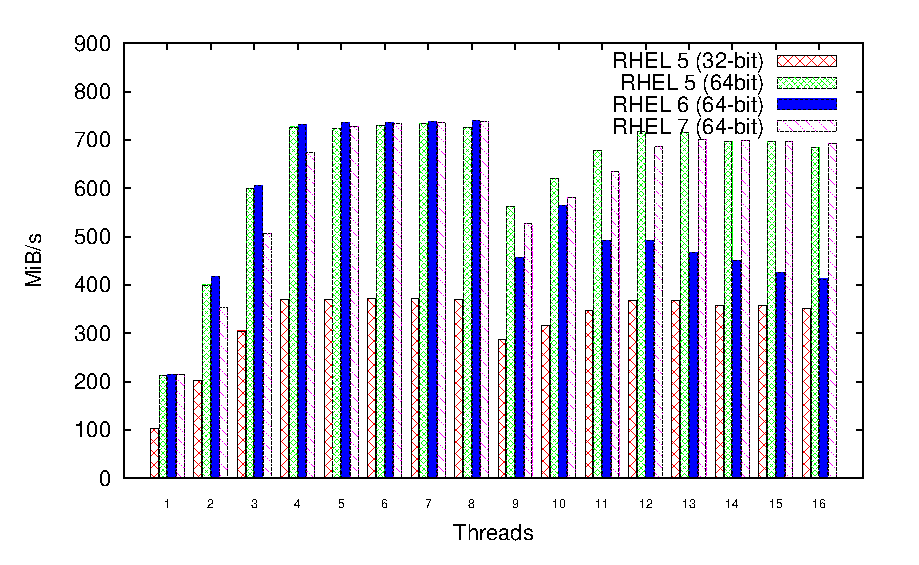
\includegraphics[width=15cm]{fig/tests/difference.eps} % Or .pdf
%\includegraphics[width=10cm,keepaspectratio]{fig/ISK-scheme}
\caption{The differences between 32 and 64-bit of RHEL 5 and RHEL 7 installation.}
\label{fig:testing:difference}
\end{figure}


%..............................................................................
\subsection{Size dependency}
\begin{tabular}{|l|c|l|}
 \hline
 OS & Arch. & Machine \\
 \hline
  \hline
 RHEL 7 & x86\_64 & \machine{hp-aladdin-01.lab.bos.redhat.com}\\
 \hline
\end{tabular}

In this test, functions \function{rdrand_get_bytes_retry} and \function{rdrand_get_uint64_array_retry} were compared in different sizes of the memory area that was filled with random numbers. The used command is {\tt ./RdRand -m METHOD -t 1 -c SIZE} -- the test was done with a single thread. For a better visibility, the figure is splitted to two parts. The \figref{fig:testing:bytesArrayHi} shows the difference from 8192 down to 64 of 64-bit numbers (quadwords) and \figref{fig:testing:bytesArrayLow} shows the rest, from 32 to just 1 generated number.

\begin{figure}[h!]
  \centering
 \includegraphics[width=12cm]{fig/tests/bytes_array_speed_low.eps} % Or .pdf
%\includegraphics[width=10cm,keepaspectratio]{fig/ISK-scheme}
\caption{The difference of two functions on different sizes of filled memory area, from 32 to 1 quadword.}
\label{fig:testing:bytesArrayLow}
\end{figure}

\begin{figure}[h!]
  \centering
 \includegraphics[width=12cm]{fig/tests/bytes_array_speed_hi.eps} % Or .pdf
%\includegraphics[width=10cm,keepaspectratio]{fig/ISK-scheme}
\caption{The difference of two functions on different sizes of filled memory area, from 8192 to 64 quadwords.}
\label{fig:testing:bytesArrayHi}
\end{figure}

On these figures it is apparent that there is a small difference between these two values in range from very few quadwords up to about one thousand of quadwords. The difference is caused by the little higher overhead in the memory align checks in \function{rdrand_get_bytes_retry}. On very small sizes, the overhead of the test itself is too big in comparison with the difference and thus these results are not reliable. However, with regard to the implementation it is probable that the difference there still is.

On the opposite side of the figures the performance difference dismiss as with big memory areas, the overhead in the logic of the function is fractional in comparison with time spend on the RdRand instruction itself.

%..............................................................................
%\pagebreak
\subsection{Fast and secure generating}\label{subsec:testing:fastVsSecure}
\begin{tabular}{|l|c|l|}
 \hline
 OS & Arch. & Machine \\
 \hline
  \hline
 RHEL 7 & x86\_64 & \machine{hp-aladdin-01.lab.bos.redhat.com}\\
 \hline
\end{tabular}

Because the secure methods, described in the section \ref{subsec:api:secure}~\nameref{subsec:api:secure} (both functions \function{rdrand_get_uint64_array_reseed_delay} and its {\tt \_skip} twin), should not be used in parallel threads\footnote{See \ref{subsec:api:secure}}, only a single thread comparison between them and the \function{rdrand_get_bytes_retry} as a fast method was made. \TODO{Data from another machine that has different delay/skip.} The values are average from few manual runs.

\begin{table}[h!]
\begin{center}
\begin{tabular}{|l|c|c|}
  \hline
 Function / Machine & \machine{hp-aladdin-01.lab.bos.redhat.com} & xx\\
  \hline
  Fast & xxx MiB/s & xx MiB/s\\ 
  \hline
  Delay & xxx MiB/s & xx MiB/s\\
  \hline
  Skip & xxx MiB/s & xx MiB/s\\
  \hline
\end{tabular}
\caption{Comparison of speed of a fast method of generating ({\tt rdrand\_get\_bytes\_retry}) and two variants of secure generating.}
\label{tab:testing:fastAndSecure}
\end{center}
\end{table}


%\pagebreak
\subsection{Performance on an unaligned memory space}
\subsection{Half performance on some machines}

\subsection{Underflow}
The only machine on which I was able to achieve underflow of the HW RNG is \machine{dell-pr1700-02.lab.bos.redhat.com}.


%------------------------------------------------------------------------------
\section{Specifications of referenced machines}
\TODO{More HW description} % TODO More HW description.

\machineDeclare{dell-pr1700-02.lab.bos.redhat.com}{Intel(R) Xeon(R) CPU E3-1285 v3 @ 3.60GHz}{Dell Precision T1700, 4 GB RAM. The internal RNG was not able to handle more than four parallel threads at November 2013.}


\machineDeclare{hp-aladdin-01.lab.bos.redhat.com}{Intel(R) Core (TM) i7-3920XM CPU @ 2.90GHz}{HP elitebook 8770w, 4 GB RAM}



%=========================================================================